% !Mode\dots ``TeX:UTF-8''
% !TEX root = ../root.tex
\section{Introction}
\label{sec:intro}
In 1960s, Nobel Prize winners Jacob and Monod found that  ``Any cell contains a number of `regulatory' genes that act as switches and can turn one another on and off. If genes can turn one another on and off, then you can have genetic circuits.'' \cite{Jacob1961Genetic}. Inspired by these Boolean-type actions in genetic circuits, the Boolean networks (\BNs) is firstly proposed by Kauffman \cite{Kauffman1968Metabolic} for modeling nonlinear and complex biological systems. Some general descriptions of the \BNs\ and its applications to biological systems can be found in \cite{Kauffman1968Metabolic}. Since then research interests in  \BNs\ have been motivated by the large number of natural and artificial systems. These systems describing variables display only two distinct configurations, and hence these describing variables take only two values, i.e., $\{0,1\}$  \cite{Akutsu2000Inferring, Shmulevich2002From, Faur2006Dynamical,Green2007The,Lou2010Multi,Fornasini2013Observability}.


When external regulation or perturbation is considered, \BNs\ are naturally extended to Boolean control networks (\BCNs) \cite{Ideker2001A}. The \BCNs\ can be used to solve various important realistic problems. For instance, first \BCNs\ have been used to do structural and functional analysis of  signaling and regulatory networks \cite{Kaufman1999A, Klamt2006A}. Second \BCNs\ have been used for abduction based drug target discovery \cite{Biane2017Abduction}. Furthermore, \BCNs\ also have been used for pursuit evasion problems in polygonal environments \cite{Thunberg2011A}. For a better understanding, we make a brief introduction about how to use \BCNs\ to do signaling and regulatory networks' structural and functional analysis. Evolution has equipped cells with exquisite signaling systems which allow them to sense their environment. The immune system is a very important part of the signaling system, it can identify and eliminate foreign invading antigens. T-cells known as lymphocytes are a type of white blood cells, they play a central role in the immune system. T-cells can recognize protentially dangerous agents for cells and initiate an reaction against these agents. T-cells do so by T-cell receptors to detect foreign antigens bound to major histocompatibility complex molecules, and then activate, through a signaling cascade, several transcription factors. As the interaction of the antigen-specific receptor of T-cells with its antigenic ligand can lead either to cell activation (1) or to a state of profound unresponsiveness (0). There are some work  apply the \BCNs\ to study the T-cell receptor kinetics model better \cite{Kaufman1999A, Klamt2006A}. The events of T-cell receptor sianaling system can be depicted as nodes in the \BCN. Except the state-nodes, the input-nodes represent the controllable events, the output-nodes represent the events to be observed. And the updating rules of the \BCN\ represent the interation of these events. The example given in \cite{Kaufman1999A} is as follows.
 \begin{example}The model shown in Fig.\ref{fig:6} consists of a series of events, each event requires a time step to be realized. For example, the event positive signaling is depicted as a state-node (Positive signaling, s). The input-node (Free ligand, f) of this \BCN\ is the controllable node, as we can control the event free ligand. The output-node is the node to be observed (PTK activity, k), as we would observe the event protein tyrosine kinase (PTK) activation. The positive action (influence) of the protein tyrosine kinase (PTK) activation on itself is depicted as the directed edge from the node (PTK activity, k) to itself. And the updating rule of the node (PTK activity, k)  
 \[k(t+1)=b(t)\vee (k(t)\wedge\neg s(t) )\] 
 describes all influence to the event protein tyrosine kinase activation. The influence come from the events binding of free ligand to T cell receptors, positive signaling and protein tyrosine kinase activation itself. For more details, we refer the readers to read \cite{Kaufman1999A, Klamt2006A}. 
\end{example}  


%By this method, we can study the properties of the 
 \begin{figure}[thpb]
      \centering
      \framebox{\parbox{3in}{
		\centerline{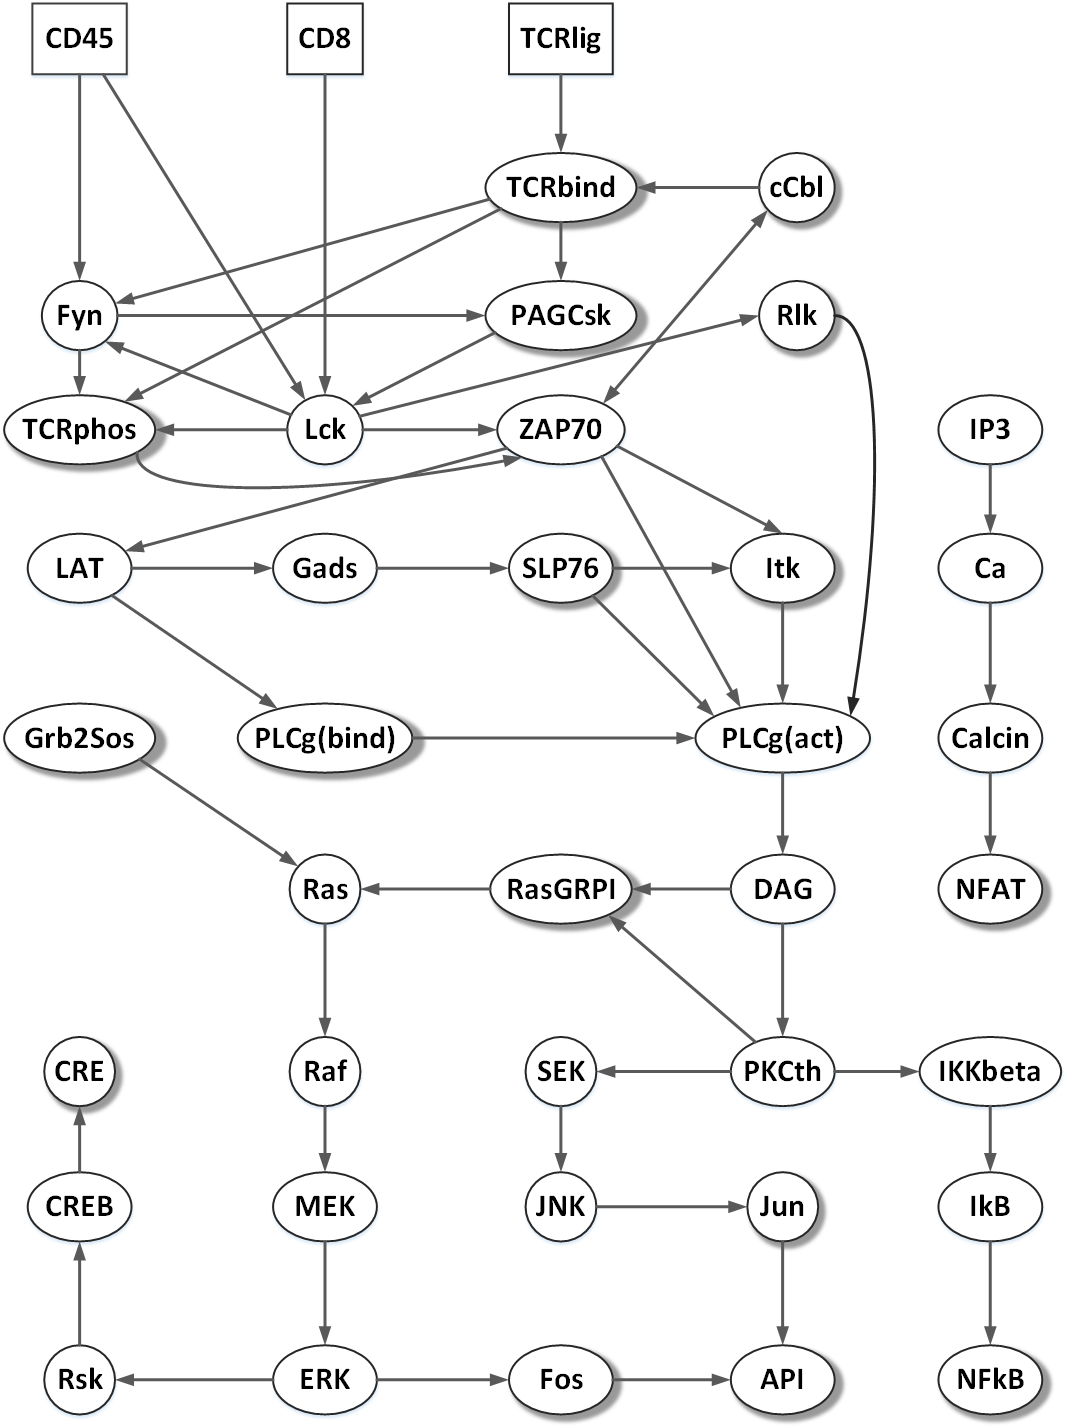
\includegraphics[scale=0.277]{figures/Fig6.png}}
	}}
      
      \caption{Schematic interaction diagram. f = free ligand; b = TCRs
bound to ligand; k = receptor-associated PTK activity; x = tyrosine
kinase-dependent inhibitory pathway; s = metabolic and mitogenic
response. Positive and negative interactions are indicated by a plus and
minus sign, respectively.}
      \label{fig:6}
  \end{figure}

As the wide application of \BCNs, there are much research work about the control-theoretic problems of \BCNs\ began with 2007 \cite{Akutsu2007Control}. The work in \cite{Akutsu2007Control} also proves that the problem of determining the controllability of \BCNs\ is {\em NP}-hard in the number of nodes. In addition, it points out that ``One of the major goals of systems biology is to develop a control theory for complex biological systems.'' The study on control-theoretic problems in the areas of \BNs\ and \BCNs\ has drawn great attention \cite{cheng2009controllability, Zhao2010Input, Cheng2011Identification, Cheng2011Analysis,Fornasini2013Observability}. Besides controllability, observability is an another  attractive basic control-theoretic problem.  Among these studies, \emph{semi-tensor product} (STP) is one of useful tools to deal with  both \BNs\ and \BCNs\  related problems \cite{cheng2009controllability}.  We will refer to STP in the following. Moreover,  the concept of \BCN\'s observability was proposed firstly in \cite{cheng2009controllability}. To date, there are four types of observability have been proposed. 
%Moreover,  \cite{cheng2009controllability} gives equivalent conditions for controllability of \BCNs\ and observability of controllable \BCNs. 
\begin{enumerate}
	\item The first type of observability proposed in 2009 \cite{cheng2009controllability} means that every initial state can be determined by an input sequence.
	
	\item 
	The second observability proposed in 2010 \cite{Zhao2010Input} stands that for every two distinct initial states, there exists an input sequence which can distinguish them, and this observability is determined in \cite{Li2015Controllability}.
	
	\item The third observability proposed in 2011 \cite{Cheng2011Identification} states that there is an input sequence that determines the initial state.
	
	\item  The fourth observability proposed in 2013 \cite{Fornasini2013Observability} is essentially the observability of linear control systems, i.e., every sufficient long input sequence can determine the initial state.
\end{enumerate}
 

%\tl{can you state the four types observability clearly and formally here?}

%\rev{****input s equence***}

In above mentioned definitions an input is not the value of an input-node of the \BCN, but it represents the values of all input-nodes of the \BCN\ on a time step. Therefore, an input can be seen as a vector of the values of all input-nodes of the \BCN\ on a time step. An input sequence consists of several inputs in sequential time steps. In every time step, there is a pair of input and output of \BCN.
     A output can be seen as a vector of the values of all output-nodes of the \BCN\ in a time step as well. Therefore a output sequence also consists of several outputs in sequential time steps. In {\em Section \ref{sec:pre}}, we will list the informal definition of four offline  observabilities as well as the formal definition of four observabilities.% in the following pages. What's more, there is an approach to study large-scale \BCNs\ via network aggregations \cite{Zhang2017Observability}. In order to further improve the performance of the \BCN\ model, we make some optimizations about the definition of observability of \BCNs.     which can be checked at most once


The four  types of observability  have many nice properties that they can be used in some useful applications. However, all of four  types of observability of \BCNs\ are offline observabilities which means that they can not adjust the input sequence by observing the output sequence in the process of determining the initial state of \BCNs. This property of offline observability limits the performance of \BCNs. In order to further improve the performance of \BCNs, we propose the online observability that we can determine the initial state of \BCNs\ dynamically. In other words,  the online observability decides the input sequence in each time step by observing the out sequence. In the  online observability, we infer the possible  initial states set by observe outputs of \BCN\ in the first $k$ time steps. Through the  possible  initial states, we can choose one input to refine the possible initial states set in the time step $k+1$. We repeat above procedure until the cardinality of initial states set turns into be one then we can determine the initial state of \BCNs. That is why we call this process a dynamic process. 

\subsubsection*{Contribution}
Firstly, we propose the concept of the online observability of \BCNs. Compared with four existing observabilities, the online observability can help us to determine the initial state of some biological systems. Secondly, in addition to theoretical research, we also provide two algorithms to determine the online observability for \BCNs. Finally, we introduce some applications of the online observability of \BCNs. Including methods to find shortest path and approaches to avoid entering critical states in the process of determining the initial state of \BCNs, etc.  These applications further explain the advantages of online observability of \BCNs\ compared with offline observabilities. %\rev{No important points}%\rev{***Compare with offline observabilities****} 
\subsubsection*{Structure}
The remainder of this paper is organized as follows. {\em Section \ref{sec:pre}} introduces necessary preliminaries about \BCNs, algebraic forms of \BCNs\ and the four existing kinds of observability of  \BCNs. {\em Section \ref{sec:online}} presents the definition of deduction function, $k$ steps determinability and online observability of \BCNs. {\em Section \ref{sec:deter}} presents how to determine the online observability of \BCNs\ by super tree and directed graph. {\em Section \ref{sec:app}} talks about some applications of the online observability of \BCNs. We also compare the online observability with offline observabilities in this section. {\em Section \ref{sec:con}} ends up  with the introduction of our future work.

%\tl{I will try to rewrite the intro.}

%==============================================================================================================